
In this section we will to every Legendrian knot ( or more acuratly the
Legendrian projection ) assosiate a finite \Ainf-algebra. This contruction
directly corresonds to the Chekanov-Eliashberg DGA constricted in
(\cite{chekanov02}).

Let $L$ be a Legendrian knot in the standard contact structure on $\R^3$.

\subsection{The vector space}
\begin{defn}
$L$ is sad to be \wddef{generic} wrt. $\pi$, if the set of crossings in $\pi(L)$
is finite and consist of transversal double points. More precisely, if $c\in
\pi(L)$ is a crossing. Then $\pi^{-1} \cap L = \{ c^+, c^- \}$ and if $T^\pm$
is the tangent line of $L$ at $c^\pm$, then $\pi(T^+) \cap \pi(T^-) = \{c\}$.
\end{defn}

For the rest if this paper will assume $L$ is generic and let $Y = \pi(L)$. ( Note that, any Legendrian knot is $C^\infty$-close to a generic one,
ie. there exist a smooth one parameter family of Legendrian knots $\{L_\alpha
\}\alpha \in [0,1]$, such that $L = L_0$ and $L_\alpha$ is generic for $\alpha >
0$. ) 

\begin{defn}
Let $\Cc = \{ a_1, \dots, a_n\}$ denote the set of double points in $Y$ and
$A = \Z_2\left<\Cc\right>$, be the $\Z_2$-vector space generated by $\Cc$.
\end{defn}

This vector space will be the base space, for the \Ainf-algebra. The grading 
on the vector space will take values in the cyclic group $\Gamma = \Z / m(L) \Z$, 
where $m(L)$ is twice the rotation number of $L$. To define the grading on the
vector space we will define the grading on each of crossing $c \in \Cc$, by the  
the rotation number of the path from $c_+$ to $c_-$ along $L$.

\begin{defn}
\label{def:theta_map}
Let $x, y \in L$ be distinct, then there are two paths from $x$
to $y$ along $L$ (that is up to re-parametrization, and such that the path
does not go around $L$ multiple times, ie. $L$ is not contained in the image
of the path).

Let $\gamma_1, \gamma_2: [0,1] \to L$, be parametrizations of these two paths.
Then $\gamma_1 * (-\gamma_2)$ is a parametrization of $L$ (where $*$
denotes concatenation), so $r(\gamma_1) - r(\gamma_2) = r(L)$.

Define $\theta: L \times L \to \R / m(L) \Z$, by 
\[ \theta(x,y) = 2 r(\gamma_1) = 2 r(\gamma_2) \mod m(L),  \]
where $m(L) = 2r(L)$. (See figure (\ref{fig:grading}))
\end{defn}

Note that $\theta$ is anti-symmetric and satisfies, $\theta(x,y) +
\theta(y,z) = \theta(x,z)$, for all $x,y,z \in L$.

Consider a crossing $c \in \Cc(Y)$, then since we assumed $L$ is generic wrt.
$\pi$, there exists unique $c_+, c_- \in L$, such that $\pi(c_+) = \pi(c_-) =
c$ and $z(c_+) > z(c_-)$, where $z(c)$ denotes the $z$-component of $c$ in $\R^3$.
We define the grading of $c$, by 
\[ |c| = \lceil \theta(c^+, c^-) \rceil \in \Z / 2r(L) \Z. \]

\figpdf{.4}{grading}{Gaussian map}

\subsection{Admissible immersions}
Before defining the \Ainf-maps, we need to define some combinatorial objects,
used to define them.

For $k \in \N$, let $\Pi_k \subset \R^2$ be a convex $k$-gon, like in figure
\pref{fig:k_gons}, with vertices $x^k_0, ..., x^k_{k-1}$ numbered anticlockwise.

\figpdf{.4}{k_gons}{$k$ sided (curved) polygon.}

\begin{defn}
Let $W_k(Y)$ be the set of orientation-preserving immersions $u: \Pi_k \to \R^2$, 
such that $u(\partial \Pi_k) \subset Y$, where $\partial \Pi_k$ denotes the
boundary of $\Pi_k$. 

Let $\Diff^*(\Pi_k)$ be the group of
orientation-preserving diffeomorphisms of $\Pi_k$ fixing the vertices, ie. the
set of re-parametrisations of $\Pi_k$. Then we define 
\[ \tilde{W_k}(Y) = W_k / \Diff^*(\Pi_k), \]
the set of non-parametrized immersions. 
\end{defn}
Note that if $u \in W_k(Y)$, then $u(x^k_i) \in \Cc$ is a crossing in $Y$ and inner
angle is less then $\pi$. 

Let $u\in \tilde{W_k}(Y)$ and consider
a small neighbourhood $U \subset \R^2$ of the crossing $u(x^k_i) \in \Cc$. Then
$Y$ divides $U$ into four quadrants. See figure \pref{fig:quad_sign}. Exactly
one of this quadrants is then covered by a neighbourhood $V \subset \Pi_k$ of
$x^k_i$.

Let $c_+, c_- \in L$, such that $\pi(c_+) = \pi(c_-) = u(x^k_i)$ and
$z(c_+) > z(c_-)$. Consider a short path $\phi: I_\epsilon= (-\epsilon,
\epsilon) \to L$, such that  
$\pi(\phi(0)) = u(x^k_i)$, $\pi(\phi(I_\epsilon)) \subset u( U\cap \partial
\Pi_k)$ and going anticlockwise through the crossing ( that is anticlockwise
around the quadrant covered by $u$). Then either 
\[ \lim_{x\to 0^\pm} \phi(x) = c_\pm \qq{\text{or}} \lim_{x\to 0^\pm} \phi(x) =
c_\mp. \] 
In the first case the z-component of $\phi$ increase going through the crossing
and in the second case it decreases. This is clearly only dependent on the
crossing and which quadrant is covered, so we may associate the signs with the
quadrants as shown in figure \pref{fig:quad_sign}. 

\begin{defn}
Let $u \in \tilde{W}_k(Y)$, if a neighbourhood of $x^k_i$ is mapped to a positive
(resp. negative) quadrant, we say, \wddef{$x^k_i$ is positive (resp. negative)
for $u$.}

An immersion $u \in \tilde{W}_k(Y)$ is called \wddef{admissible}, if $x^k_0$ is
positive for $u$ and $x^k_i$ is negative for $u$, for all $i \ge 1$.
Let
\[ W_k^+(Y) = \{ u \in \tilde{W}_k(Y) \q| u \text{ is admissible} \}. \]
If $a \in \Cc$, we write 
\[ W_k^+(Y,a) = \{ u \in W_k^+(Y) \q| u(x^k_0) = a \}. \]
\end{defn}

\begin{lemma}
\label{prop:W_+_finite}
$W^+_k(Y)$ is finite.
\end{lemma}
The proof will be covered in the following chapter.

\begin{figure}[ht]
  \centering
  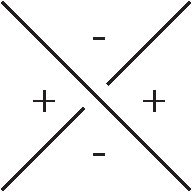
\includegraphics[width=.4\textwidth]{figs/cornerasy.pdf}
  \caption{Quadrants near a crossing in $\pi(L).$}
  \label{fig:quad_sign}
\end{figure}

\subsection{The \Ainf-maps $m_k$}
\label{sect:Ainf_m}
% Now we mey define the \Ainf-maps.

Fix $k$, and let $a, b_1, ...,  \in \Cc$, then denote
\[ \M^a_{b_1...b_k} = \{ u \in W^+(Y,a) \q|  u(x^k_i) = b_i \text{ for } i\ge 1 \}. \]
Then define
\[ m_k(b_1, ..., b_k) := \sum_{a\in\Cc} (\#_2 \M^a_{b_1...b_k}) a, \]
where $\#_2$ denotes the number of elements modulo 2, which is well-defined, by
lemma \pref{prop:W_+_finite}.

\begin{them}[Chekanov 2002, \cite{chekanov02}]
\label{prop:a_inf_rels}
The maps $m_k$ have degree $2-k$ and satisfies the curved $A_\infty$-relations,
ie. $\forall n\ge 0$,
\begin{equation}
\label{eq:a_inf_rel}
\xi_n := 
\sum_{r+s+t = n} m_u(\I^{\otimes r} \otimes m_s \otimes \I^{\otimes t})  = 0,  
\end{equation}
where $u = r+1+t$. Hence, by lemma \pref{prop:W_+_finite}, $(A,m_i)$ defines a
finite curved $A_\infty$-algebra.
\end{them}

\begin{them}[Chekanov 2002, \cite{chekanov02}]
\label{prop:stable_tame_inv}
Let $(A,m)$ and $(A', m')$ be the \Ainf-algebras associated to Legendrian knots $L$ and $L'$. Then if $L$ and $L'$ differ by a Legendrian isotopy, $(A,m)$ and $(A',m')$ have the same sable type.
%are related by a stable tame isomorphism.
\end{them}

The proofs of these theorems are given in chapter \ref{chap:proofs}.

